\section{Introduction}

% What is the problem?
File system metadata services in HPC and large-scale data centers have
scalability problems because common tasks, like
checkpointing~\cite{bent_plfs_2009} or scanning the file
system~\cite{zheng:pdsw2014-batchfs}, contend for the same directories and
inodes. Applications perform better with dedicated metadata
servers~\cite{sevilla:sc15-mantle, ren:sc2014-indexfs} but provisioning a
metadata server for every client is unreasonable. This problem is exacerbated
by current hardware and software trends; for example, HPC architectures are
transitioning from complex storage stacks with burst buffer, file system,
object store, and tape tiers to more simplified stacks with just a burst buffer
and object store~\cite{bent:login16-hpc-trends}. These types of trends put
pressure on data access because more requests end up hitting the same layer and
latencies cannot be hidden while data migrates across tiers.

% What is HPC doing?
To address this, developers are relaxing the consistency and durability
semantics in the file system because weaker guarantees are sufficient for their
applications. For example, many batch style jobs do not need the strong
consistency that the file system provides, so
BatchFS~\cite{zheng:pdsw2014-batchfs} and DeltaFS~\cite{zheng:pdsw2015-deltafs}
do more client-side processing and merge updates when the job is done.
Developers in these domains are turning to these non-POSIX IO solutions because
their applications are well-understood ({\it e.g.}, well-defined read/write
phases, synchronization only needed during certain phases, workflows describing
computation, etc.) and because these applications wreak havoc on file systems
designed for general-purpose workloads ({\it e.g.}, checkpoint-restart's N:N
and N:1 create patterns~\cite{bent_plfs_2009}).

\begin{figure}[tb] \centering
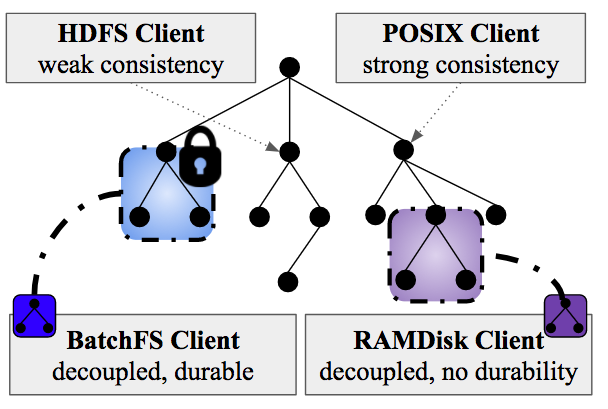
\includegraphics[width=0.35\textwidth]{figures/subtree-policies1.png}
\caption{Illustration of subtrees with different semantics co-existing in a
global namespace.  For performance, clients can relax consistency on their
subtree (HDFS) or decouple the subtree and move it locally (BatchFS, RAMDisk).
Decoupled subtrees can relax durability for even better performance.
}\label{fig:subtree-policies} \end{figure}

% One example
One popular approach for relaxing consistency and durability is to ``decouple
the namespace", where clients lock the subtree they want exclusive access to as
a way to tell the file system that the subtree is important or may cause
resource contention in the near-future~\cite{grider:pdsw2015-marfs,
zheng:pdsw2015-deltafs, zheng:pdsw2014-batchfs, ren:sc2014-indexfs,
bent:slides-twotiers}. Then the file system can change its internal structure
to optimize performance. For example, the file system could enter a mode that
prevents other clients from interfering with the decoupled directory.  This
delayed merge ({\it i.e.} a form of eventual consistency) and relaxed
durability improves performance and scalability by avoiding the costs of remote
procedure calls (RPCs), synchronization, false sharing, and serialization.
While the performance benefits of decoupling the namespace are obvious,
applications that rely on the file system's guarantees must be deployed on an
entirely different system or re-written to coordinate strong
consistency/durability themselves.

% What did we do
To address this problem, we present an API and framework that lets developers
dynamically control the consistency and durability guarantees for subtrees in
the file system namespace.  Figure~\ref{fig:subtree-policies} shows a potential
setup in our proposed system where a single global namespace has subtrees for
applications optimized with techniques from different state-of-the-art
architectures.  The HDFS\footnote{HDFS itself is not directly evaluated in this
paper, although the semantics and their performance is explored
in~\S\ref{sec:use-case-1}.} subtree has weaker than strong consistency because
it lets clients read files opened for
writing~\cite{hakimzadeh:dais14-hdfs-consistency}, which means that not all
updates are immediately seen by all clients; the BatchFS and RAMDisk subtrees
are decoupled from the global namespace and have similar consistency/durability
behavior to those systems; and the POSIX IO subtree retains the rigidity of
POSIX IO's strong consistency.  Subtrees without policies inherit the
consistency/durability semantics of the parent and future work will examine
embeddable or inheritable policies.

Our prototype system, Cudele, achieves this by exposing ``mechanisms" that
users combine to specify their preferred semantics.  Cudele supports 3 forms
of consistency (invisible, weak, and strong) and 3 degrees of durability (none,
local, and global) giving the user a wide range of policies and optimizations
that can be custom fit to an application. We make the following contributions:

\begin{enumerate}

  \item A framework and API for assigning consistency/durability policies 
  to subtrees in the file system namespace; this lets users navigate
  the trade-offs of different metadata protocols on the same storage system.

  \item This framework lets subtrees with different semantics co-exist in a
  global namespace. We show how this scales further and performs better than
  systems that use one strategy for the entire namespace .

  \item A prototype that lets users custom fit subtrees to applications
  dynamically. 

\end{enumerate}

\oldcomment{The last contribution lays the groundwork for future work on our
prototype. It is more scalable than the current practice of mounting different
storage systems in a global namespace because there is no need to provision
dedicated storage clusters to applications or move data between these systems.
For example, the results of a Hadoop job do not need to be migrated into a Ceph
file system (CephFS) for other processing; instead the user can change the
semantics of the HDFS subtree into a CephFS subtree.  This may cause
metadata/data movement to make things strongly consistent again but this is
superior to moving all data across file system boundaries. Our prototype
enables studies that adjust these semantics over {\it time and space}, where
subtrees can change their semantics and migrate around the cluster without ever
moving the data they reference.}

% Results
The results in this paper pave the way for such a system and confirm the
assertions of ``clean-state" research of decoupled namespaces; specifically
that these techniques drastically improve performance.  We go a step further by
quantifying the costs of merging updates (3.37\(\times\) slowdown) and
maintaining durability (\(2.4\times\) slowdown).  In our prototype,
\newcomment{we also show how to assign subtree semantics for certain
applications such as checkpoint-restart (\(91.7\times\) speedup if consistency
is fully relaxed), user home directories (within a 0.03 standard deviation from
optimal), and clients checking for partial results (only a 2\% overhead).}
\oldcomment{we get an 8\(\times\) speedup and can scale to twice as many
clients when we assign a more relaxed form of consistency and durability to a
subtree with a create-heavy workload.}  We use Ceph as a prototyping platform
because it is used in cloud-based and data center systems and has a presence in
HPC~\cite{wang:pdsw13-ceph-hpc}.

%In the remainder of the paper, Section~\ref{sec:posix-overheads} quantifies the
%cost of POSIX IO consistency and system-defined durability and
%Section~\ref{sec:methodology-decoupled-namespaces} presents the Cudele
%prototype and API. Section~\ref{sec:implementation} describes the Cudele
%mechanisms and shows how re-using internal subsystems results in an
%implementation of less than 500 lines of code. The evaluation in
%Section~\ref{sec:evaluation} quantifies the overheads and performance gains of
%explored and previously unexplored metadata designs.
%Section~\ref{sec:related-work} places Cudele in the context of other related
%work.

